\section{Maschinelles Lernen}
\setauthor{Lukas Starka}


\section{Deep Learning}
\setauthor{Lukas Starka}


\section{Neuronale Netze}
\setauthor{Lukas Starka}
\subsection{Convolutional Neural Networks}
\setauthor{Lukas Starka}

\subsection{Recurrent Neural Networks}
\setauthor{Lukas Starka}


\section{Word Vectors}
\setauthor{Lukas Starka}


\section{Text Analysis}
\setauthor{Lukas Starka}

\subsection{Text analysis vs. Text Mining vs. Text Analytics}
\setauthor{Lukas Starka}

Meistens werden die Begriffe Text Analysis und Text Mining im selben Zusammenhang verwendet.
Dabei bedeuten sie eigentlich dasselbe, nämlich, dass man den Sinn einer Nachricht extrahiert.
Deswegen wird in den folgenden Kapiteln nur von Text Analysis gesprochen.

Es gibt jedoch einen Unterschied zwischen Text Analysis und Text Analytics.
Grundsätzlich kann man dabei sagen, dass Text Analysis qualitative Ergebnisse liefert, wohingegen bei Text Analytics die Quantität mehr im Vordergrund steht.\cite{textAnalysisMonkeylearn, machineLearningTextAnalysis}

Bei Text Analysis werden also wichtige Informationen aus der Nachricht herausgelesen.
Oder anders formuliert geht es darum, dass trotz der Vielseitigkeiten der menschlichen Sprache trotzdem die Kernaussage herausgefunden werden kann, mit der dann gearbeitet wird.
Es können also dann Informationen herausgefiltert werden, wie beispielsweise, ob etwas positiv oder negativ ist oder was das Hauptthema des Textes ist.\cite{textAnalysisMonkeylearn, machineLearningTextAnalysis}

Auf der anderen Seite wird bei Text Analytics werden verschiedene Muster aus einer großen Menge an Nachrichten herausgefiltert, welche dann in Graphen, Tabellen oder Berichten gezeigt werden können.
Bei Text Analytics geht es also darum Muster und Entwicklungen von numerischen Ergebnissen herauszufinden, bei denen dann Informationen herausgefiltert werden können, wie beispielsweise, die Prozentzahl der positiven Bewertungen.\cite{textAnalysisMonkeylearn, machineLearningTextAnalysis}

\subsection{Warum Text Analysis?}
\setauthor{Lukas Starka}

Im Gegensatz zum manuellen Aufbereiten von Texten sorgt Machine Learning für eine schnelle Bearbeitung, die außerdem auch kostengünstiger ist, weil viele Stellen wegfallen, die benötigt werden würden, um die Texte selber aufzubereiten.
Durch die Verwendung von Text Analysis spart man sich viele Arbeitskräfte, die bei anderen wichtigen Aufgaben innerhalb eines Unternehmens eingesetzt werden können.
Außerdem können dadurch Texte rund um die Uhr und zur Echtzeit bearbeitet werden.
Durch Algorithmen werden außerdem Fehler reduziert, die bei manuellem Bearbeiten leicht auftreten können und Daten können genauer aufbereitet werden.\cite{textAnalysisMonkeylearn}

\subsection{Machine Learning mit Text Analysis}
\setauthor{Lukas Starka}

Grob kann man behaupten, dass ein Text Analysis Tool aus drei verschiedenen Schritten besteht.

\begin{enumerate}
    \item Zunächst muss man sich überlegen, welche Daten gesammelt werden sollen, um damit sein Modell zu trainieren und zu testen.
    Man unterscheidet hierbei zwischen "Internal Data" und "External Data".
    Unter External Data werden Quellen, wie Zeitungen oder Foren bezeichnet und zu der Internal Data zählen sämtliche Daten, die eine Firma jeden Tag generiert, wie E-Mails, Reports, Chats oder Umfragen.
    \item Danach müssen die Daten vorbereitet werden, damit das Programm diese versteht.
    Dieser Schritt wird meistens als "Data Preprocessing" bezeichnet.
    \item Zum Schluss wird dann ein Machine Learning Algorithmus hinzugefügt, welcher sich um die Analyse kümmert.
    Diesen kann man entweder komplett selber implementieren oder man nimmt sich Libraries zur Hilfe.\cite{machineLearningTextAnalysis}
\end{enumerate}

\section{Natural Language Processing (NLP)}
\setauthor{Lukas Starka}

Natural Language Processing, oft auch als Akronym \textbf{NLP} abgekürzt, sorgt dafür, dass Computer Text auf dieselbe Art und Weise verstehen, wie wir es als Menschen tun.
NLP vereint dabei die Modellierung der menschlichen Sprache mit statistischen Machine Learning und Deep Learning Modellen.
Dies ermöglicht der Maschine im Endeffekt, dass diese menschliche Sprache in Form von Text- oder Sprachdaten zu verarbeiten und sozusagen die komplette Bedeutung und Absicht der Benutzerin oder des Benutzers zu verstehen.\cite{naturalLanguageProcessingIBM}

\subsection{Corpus}
\setauthor{Lukas Starka}

Unter dem Corpus werden die Daten bezeichnet, die verwendet werden, um das NLP Modell zu trainieren, damit dieses menschliche Sprache versteht und damit arbeiten kann.
Der Textkorpus ist also eine Menge von strukturierten Texten, die für den Computer lesbar sind.\cite{corpus}


\subsection{Tokenization}
\setauthor{Lukas Starka}

Bei der Tokenization repräsentiert jeder Token eine sinnvolle Einheit.
Darunter versteht man Wörter, Zeichen oder Sonderzeichen, die alle einen eigenen Token darstellen, lediglich Leerzeichen in einem Satz stellen keine eigenen Token dar.\cite{machineLearningTextAnalysis, naturalLanguageProcessing}

Die verschiedenen Token, die dabei entstehen, können dabei wie folgt aussehen:

\begin{lstlisting}[label={lst: Tokenization}]
Let us go to the park.

0: Let
1: us
2: go
3: to
4: the
5: park
6: .
\end{lstlisting}

Die Tokenization ist dabei besonders für verschiedene Sprachen von Vorteil, da es in diesen immer andere Regeln gibt, wie die Wörter aufgeteilt werden können.
In dem obigen Beispiel wirkt es womöglich no so, als könnte man mit einer \textbf{split()} Methode das selbe Resultat erzielen, aber es gibt auch Besonderheiten einer Sprache, die vom Tokenizer bedacht werden müssen, wie folgendes Beispiel aufzeigt.\cite{machineLearningTextAnalysis, naturalLanguageProcessing}

\begin{lstlisting}[label={lst: Tokenization Ausnahme}]
"Let's go to the U.K.!"

0: "
1: Let
2: 's
3: go
4: to
5: the
6: U.K.
7: !
8: "
\end{lstlisting}

\subsection{Part-of-speech-Tagging (POS-Tagging)}
\setauthor{Lukas Starka}

Beim Part-of-speech-Tagging geht es um das Taggen von Wörtern und deren zugehörigen Teil der Sprache.
Als Teil einer Sprache, also dem Part-of-speech, werden grundsätzlich Wörter bezeichnet, die ähnliche grammatikalische Eigenschaften oder Nutzungen besitzen.
Im deutschen sind hierbei also die verschiedenen Wortarten gemeint.

Beim Tagging werden entweder Statistiken angewendet, wie beispielsweise, dass es sehr wahrscheinlich ist, dass nach einem Artikel ein Nomen folgt.
Außerdem gibt es sogenannte Rule-Based POS-Taggers, deren Aufgabe es ist, vordefinierte Regeln zu verwenden, um das Tagging zu vollziehen.\cite{machineLearningTextAnalysis, naturalLanguageProcessing}

Ein Beispiel für POS-Tagging könnte also folgendermaßen aussehen:

\begin{lstlisting}[label={lst: POS-Tagging}]
I am going to the U.K.

I: Pronoun
am: Verb
going: Verb
to: Part
the: Article
U.K.: Noun
\end{lstlisting}

\subsection{Named-entity recognition (NER)}
\setauthor{Lukas Starka}

Named-entity recognition ist eine der wichtigsten Säulen von Natural Language Processing.
Entities sind strukturierte Stücke von Informationen, die sich innerhalb der Nachricht einer Benutzerin oder eines Benutzers befinden.
Dabei werden Entities aus Texten erkannt und anschließend mit einem Tag der zugehörigen Kategorie versehen.\cite{namedEntityRecognition}

Beispiele für Entities wären also:

\begin{lstlisting}[label={lst: NER-Tagging}]
PERSON      Personen (inklusive fiktionalen Personen)
NORP        Nationalitäten oder religiöse oder politische Gruppen
FACILITY    Gebäude, Flughäfen, Brücken, Straßen
LOC         Orte
PRODUCT     Objekte, Fahrzeuge, Essen
LANGUAGE    Sprachen
\end{lstlisting}

\subsection{Stemming}
\setauthor{Lukas Starka}

Beim Preprocessing von Texten sind außerdem das Stemming und die Lemmatization Schritte, die häufig durchgeführt werden.

Beim Stemming wird der Wortstamm eines Tokens von den Präfixen und Suffixen gelöst.
Unter einem Präfix versteht man eine Vorsilbe, die dem Wortstamm vorangestellt wird und bei dem Suffix, handelt es sich im Gegenzug dazu um Worterweiterungen, die dem Stamm folgen.
Hierbei gibt es wieder die Möglichkeit selber einen Stemmer zu implementieren oder bereits vorgefertigte Stemmer zu verwenden.\cite{textAnalysisMonkeylearn, machineLearningTextAnalysis}

Ein Beispiel für Stemming wäre also wie folgt:

\begin{lstlisting}[label={lst: Stemming}]
Buying ---> buy

unpredictability ---> un + predict + able + ity
un          prefix
predict     base word
able        suffix
ity         suffix
\end{lstlisting}

\subsection{Lemmatization}
\setauthor{Lukas Starka}

Unter der Lemmatization oder auch Lemmatisierung wird der Prozess verstanden, bei dem alle verschiedenen Arten von einem Wort zu ihrem Wortstamm umgeformt werden.

Die Lemmatisierung ist sozusagen eine Weiterentwicklung des Stemming und versucht im Gegensatz zum Stemming den Kontext zu den Wörtern zu bringen.
Je nachdem in welchem Kontext die Verben gebraucht werden können sie sich dabei von ihrer Wortart unterscheiden und so eine andere Bedeutung haben.
Generell lässt sich sagen, dass Stemmer meist einfacher zu implementieren sind und für schnellere Laufzeiten sorgen, allerdings wird von vielen auch die Lemmatization dem Stemming vorgezogen, aufgrund der Vorteile die das Einbeziehen des Kontextes mit sich bringt.\cite{machineLearningTextAnalysis, textAnalysisMonkeylearn, stemmingLemmatization, }


Beispiele für die Lemmatisierung sind:

\begin{lstlisting}[label={lst: Lemmatization}]
better ---> good
walking ---> walk
walked ---> walk
walks ---> walk
meeting ---> meet (wenn es als Verb gebraucht wird)
\end{lstlisting}

\subsection{Parsing}
\setauthor{Lukas Starka}

Parsing könnte man so beschreiben, dass es eine Art ist um einen Satz auseinanderzuteilen, um die Struktur des Satzes besser zu verstehen.
Beim Parsing wird also die syntaktische Struktur eines Textes bestimmt.
Um dies zu erreichen, nimmt der Parsing Algorithmus die Eigenheiten der Grammatik, von der jeweiligen Sprache, in der der Text geschrieben ist, her.\cite{textAnalysisMonkeylearn}

Es gibt zwei verschiedene Arten von Parsing.
Diese sind das sogenannte "Dependency Parsing" und das sogenannte "Constituency Parsing".

\subsubsection{Dependency Parsing}
\setauthor{Lukas Starka}

Beim Dependency Parsing wird die grammatische Struktur eines Satzes bestimmt.
Außerdem kann man mithilfe des Dependency Parsing herausfinden, welche Wörter zusammenhängen und welche Beziehung diese zueinander aufweisen.
Dies bedeutet beispielsweise, dass man bei den Wörtern "blauer Ball", "nette Frau" oder ähnlichem erkennen kann, dass sich die Wörter "blau" oder "nett" auf das nachfolgende Wort bezieht.
Ein anderes Beispiel könnten die Wörter "black" und "car" sein.

\begin{figure}[hbt!]
    \centering
    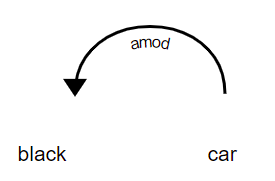
\includegraphics[scale=1]{pics/dependency_parsing}
    \caption{Beispiel für die Beziehung zweier Wörter beim Dependency Parsing~\cite{dependencyParsing}}
    \label{fig:dependency_parsing_relation}
\end{figure}

Wie man dieser Grafik entnehmen kann, bezieht sich die Farbe Schwarz in diesem Fall auf das Auto.
Im Englischen wird das Wort "car" deswegen auch als "Head" bezeichnet und "black" ist ein "child", also ein Wort, dass abhängig von diesem "Head" ist.
Die Beziehung, die zwischen diesen Wörtern vorliegt, wird mit "amod" bezeichnet.
Dies ist eine Abkürzung für "Adjectival Modifier", also ein Adjektiv, welches ein Nomen modifiziert und zu der Bedeutung des Nomens beiträgt.
In diesem Fall gibt dieses eine genaue Beschreibung der Farbe des Autos.\cite{dependencyParsing}

Diese Beziehungen kann man auch in einem Tree darstellen.

\begin{figure}[hbt!]
    \centering
    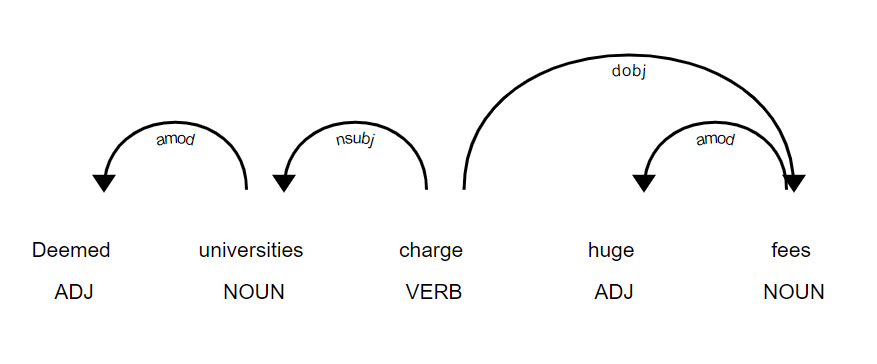
\includegraphics[scale=1]{pics/dependency_parsing_tree}
    \caption{Darstellung des Dependency Parsing~\cite{dependencyParsing}}
    \label{fig:dependency_parsing_tree}
\end{figure}

\subsubsection{Constituency Parsing}
\setauthor{Lukas Starka}


\subsection{Stopwords}
\setauthor{Lukas Starka}


\subsection{Vectorization}
\setauthor{Lukas Starka}


\subsection{Skalarprodukt}
\setauthor{Lukas Starka}

\subsection{Kreuzprodukt}
\setauthor{Lukas Starka}


\subsection{Bag of Words}
\setauthor{Lukas Starka}


\subsection{Bag of n-grams}
\setauthor{Lukas Starka}


\subsection{Vector Spaces}
\setauthor{Lukas Starka}


\subsection{Term Frequency times Inverse Document Frequency (TF-IDF)}
\setauthor{Lukas Starka}


\subsection{Zipfsches Gesetz}
\setauthor{Lukas Starka}


\subsection{Word2Vec}
\setauthor{Lukas Starka}


\subsection{NLP und NLU Tools}
\setauthor{Lukas Starka}


\subsection{NLP in Rasa}
\setauthor{Lukas Starka}

In Rasa kann man sich die verschiedenen Schritte vom Natural Language Processing ansehen, indem man sich die \hyperref[sec:pipeline]{Pipeline} ansieht.
Diese befindet sich in der \textbf{config.yml} Datei und dort sind alle Komponenten aufgelistet, die Rasa verwendet und man kann diese nach Belieben auch selbst bearbeiten.